\documentclass[10pt]{beamer}
\usetheme[
%%% options passed to the outer theme
%    hidetitle,           % hide the (short) title in the sidebar
%    hideauthor,          % hide the (short) author in the sidebar
%    hideinstitute,       % hide the (short) institute in the bottom of the sidebar
%    shownavsym,          % show the navigation symbols
%    width=2cm,           % width of the sidebar (default is 2 cm)
%    hideothersubsections,% hide all subsections but the subsections in the current section
%    hideallsubsections,  % hide all subsections
%    left                % right of left position of sidebar (default is right)
  ]{Aalborg}
  
% If you want to change the colors of the various elements in the theme, edit and uncomment the following lines
\definecolor{orangegit}{RGB}{240,80,51}

% Change the bar and sidebar colors:
\setbeamercolor{Aalborg}{fg=orangegit!20,bg=orangegit}
%\setbeamercolor{sidebar}{bg=orangegit}
% Change the color of the structural elements:
%\setbeamercolor{structure}{fg=red}
% Change the frame title text color:
%\setbeamercolor{frametitle}{fg=red}
% Change the normal text color background:
%\setbeamercolor{normal text}{bg=gray!10}
% ... and you can of course change a lot more - see the beamer user manual.

\usepackage[utf8]{inputenc}
\usepackage[portuguese]{babel}
\usepackage[T1]{fontenc}
% Or whatever. Note that the encoding and the font should match. If T1
% does not look nice, try deleting the line with the fontenc.
\usepackage{helvet}
\usepackage{hyperref}


% colored hyperlinks
\newcommand{\chref}[2]{%
  \href{#1}{{\usebeamercolor[bg]{Aalborg}#2}}%
}

\title[Uma breve apresentação]% optional, use only with long paper titles
{GIT}

\subtitle{Uma Breve Apresentação}  % could also be a conference name

\date{}

\author[Índice] % optional, use only with lots of authors
{
  Gian Lucas Cavalcante de Lima \\
}
% - Give the names in the same order as they appear in the paper.
% - Use the \inst{?} command only if the authors have different
%   affiliation. See the beamer manual for an example

\institute[
%  {\includegraphics[scale=0.2]{aau_segl}}\\ %insert a company, department or university logo
  %Dept.\ de Engenharia de Computação e Automação\\
  UFRN
] % optional - is placed in the bottom of the sidebar on every slide
{% is placed on the bottom of the title page
  %Departamento de Engenharia de Computação e Automação\\
  Universidade Federal do Rio Grande do Norte
  
  %there must be an empty line above this line - otherwise some unwanted space is added between the university and the country (I do not know why;( )
}

% specify the logo in the top right/left of the slide
\pgfdeclareimage[height=1cm]{mainlogo}{AAUgraphics/git-logo} % placed in the upper left/right corner
\logo{\pgfuseimage{mainlogo}}

% specify a logo on the titlepage (you can specify additional logos an include them in 
% institute command below
\pgfdeclareimage[height=1.6cm]{titlepagelogo}{AAUgraphics/git-icon} % placed on the title page
%\pgfdeclareimage[height=1.5cm]{titlepagelogo2}{AAUgraphics/aau_logo_new} % placed on the title page
\titlegraphic{% is placed on the bottom of the title page
  \pgfuseimage{titlepagelogo}
%  \hspace{1cm}\pgfuseimage{titlepagelogo2}
}

\begin{document}
% the titlepage
{\aauwavesbg
\begin{frame}[plain,noframenumbering] % the plain option removes the sidebar and header from the title page
  \titlepage
\end{frame}}
%%%%%%%%%%%%%%%%

% TOC
%\begin{frame}{Sumário}{}
%\tableofcontents
%\end{frame}
%%%%%%%%%%%%%%%%

\section{O que é GIT?}
\begin{frame}{Introdução}{}
\begin{block}{O que é GIT?}
  \begin{itemize}
    \item<1-> Git é um sistema de controle de versão de arquivos. Através deles podemos desenvolver projetos na qual diversas pessoas podem contribuir simultaneamente no mesmo, editando e criando novos arquivos e permitindo que os mesmos possam existir sem o risco de suas alterações serem sobrescritas.
    \item<2-> Outro fator importante do git (diferente do svn) é a possibilidade de criar, a qualquer momento, vários branch do seu projeto.
  \end{itemize}
\end{block}
\end{frame}
%%%%%%%%%%%%%%%%

\subsection{Como funciona}
% the license
\begin{frame}{Introdução}{Como funciona}
	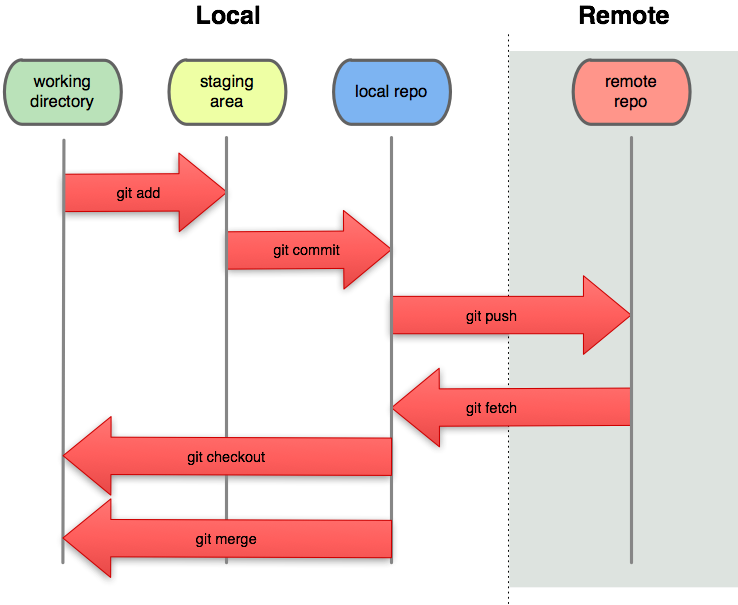
\includegraphics[scale=0.75]{AAUgraphics/funcionamento.png}  
\end{frame}
\begin{frame}{Introdução}{Como funciona}
	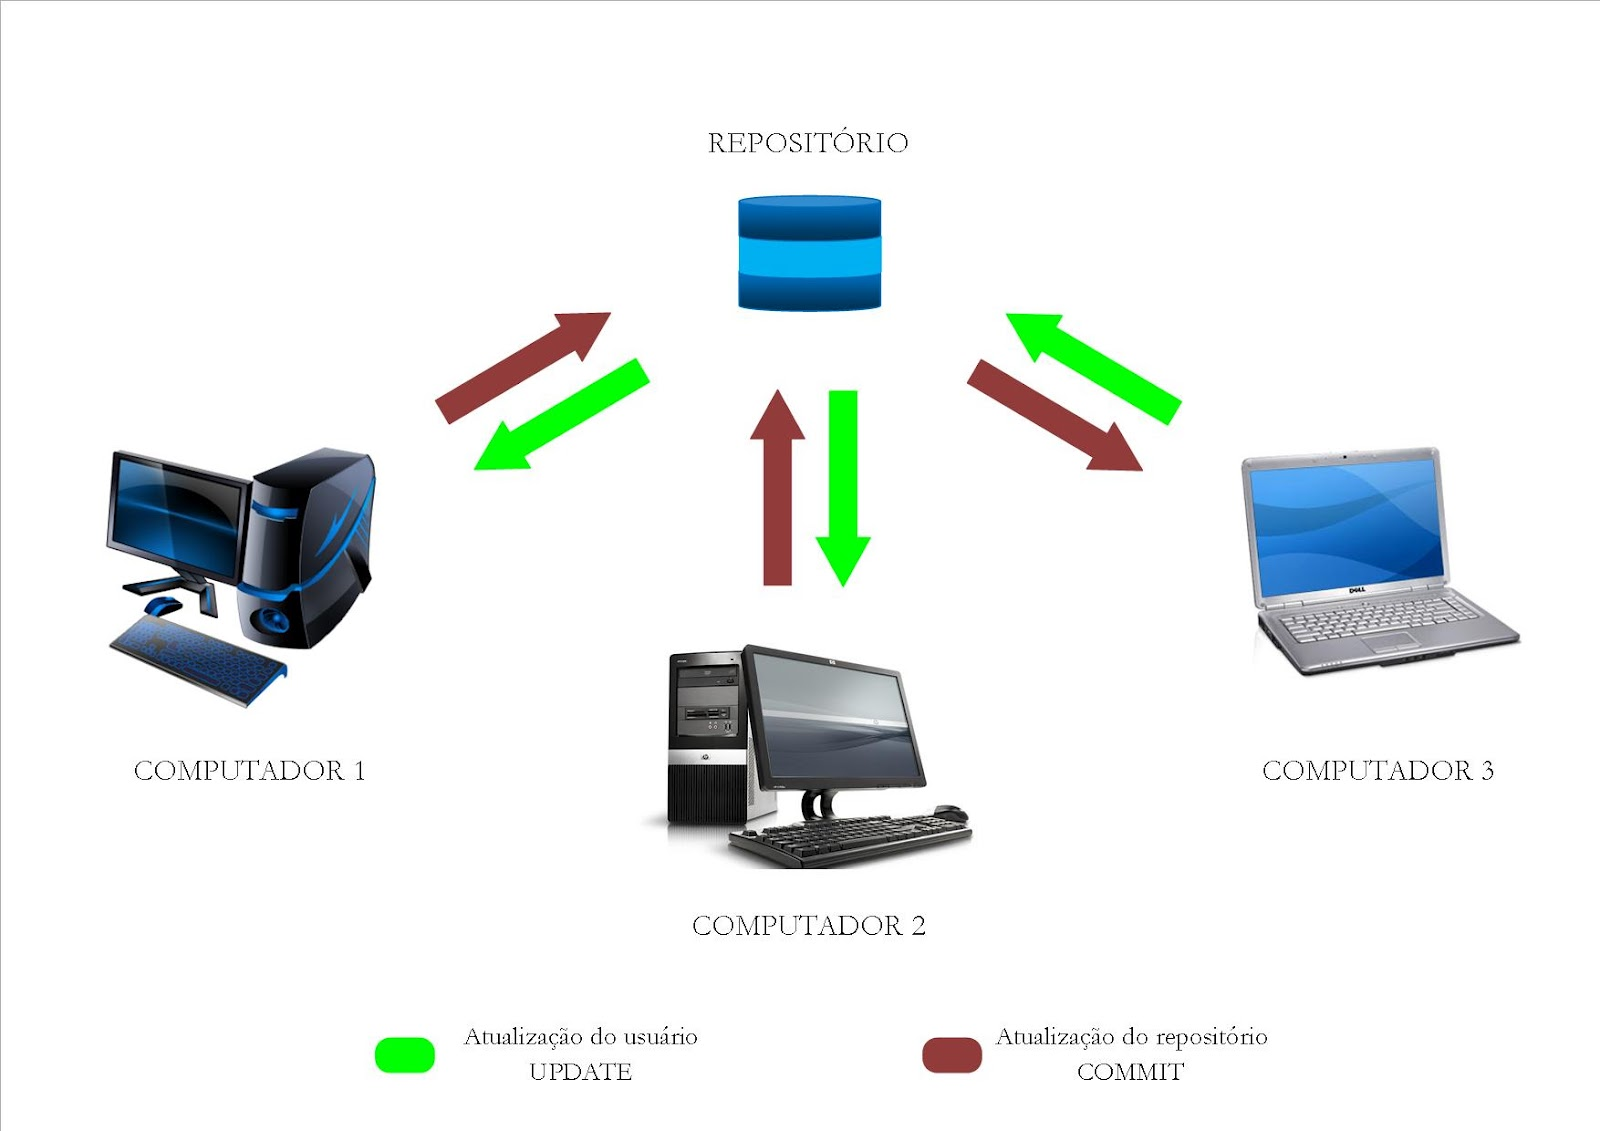
\includegraphics[scale=0.17]{AAUgraphics/esquema2}  
\end{frame}
%%%%%%%%%%%%%%%%

%\subsection{O jogo}
%\begin{frame}{Introdução}{O jogo}
%  \begin{itemize}
%    \item<1-> O objetivo do jogo é ser um jogo de memória e reflexos aonde o primeiro %jogador entra com uma sequência de 5 digitos em 3 botões e o segundo jogador deve repetir %a sequência corretamente no menor tempo possível.
%  \end{itemize}
%\end{frame}
%%%%%%%%%%%%%%%%

\section{Como Usar}
\subsection{Instalação}
% general installation instructions
\begin{frame}{Começando a usar}{Instalando no Linux}
  \begin{itemize}
  	\item Arch Linux
  	\begin{itemize}
  		\item \$ sudo pacman -S git
  	\end{itemize}
  	\item Fedora
  	\begin{itemize}
  		\item \$ sudo dnf -y update
  		\item \$ sudo dnf -y git
  	\end{itemize}
  	\item Ubuntu
  	\begin{itemize}
  		\item \$ sudo apt-get update
  		\item \$ sudo apt-get install git
  	\end{itemize}
  \end{itemize}
\end{frame}

\begin{frame}{Começando a usar}{Instalando no Windows}
  
\includegraphics[scale=0.37]{AAUgraphics/download1}
\end{frame}
\begin{frame}{Começando a usar}{Instalando no Windows}
  
\includegraphics[scale=0.32]{AAUgraphics/download2}
\end{frame}

\subsection{Registro}
\begin{frame}{Começando a usar}{Registrando a máquina}
  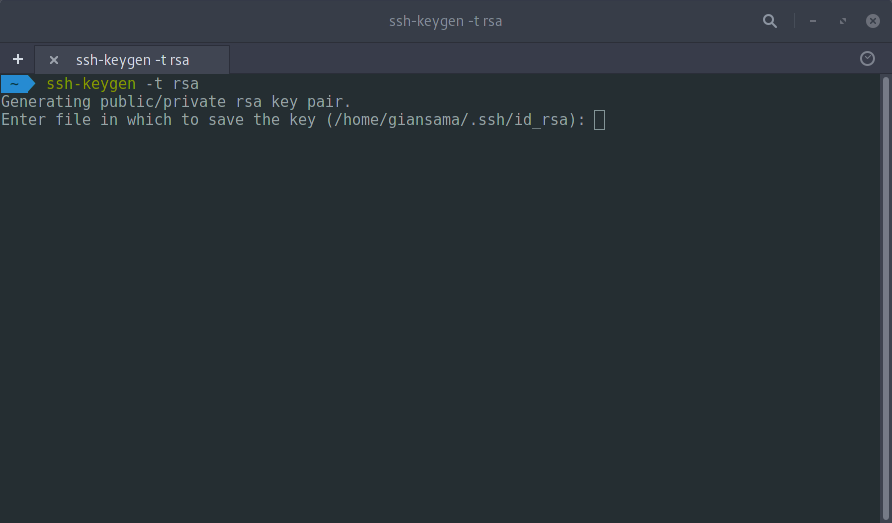
\includegraphics[scale=0.42]{AAUgraphics/ssh1}
\end{frame}
\begin{frame}{Começando a usar}{Registrando a máquina}
  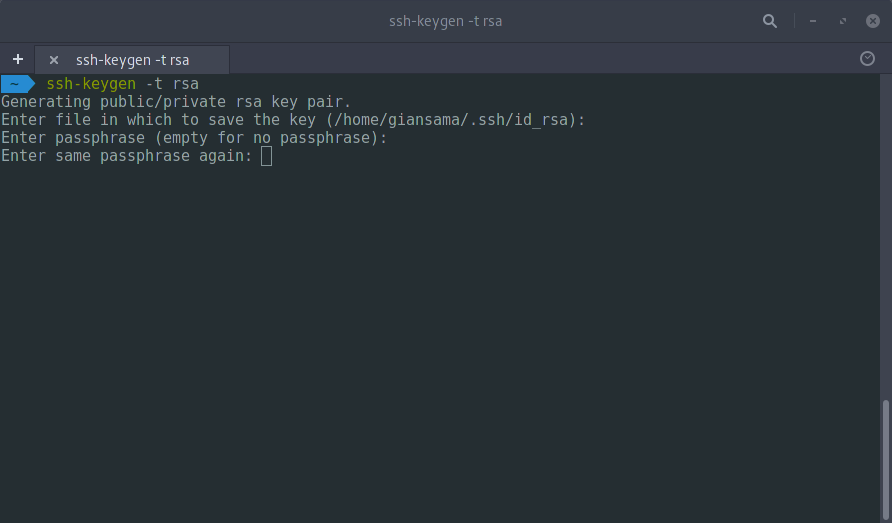
\includegraphics[scale=0.42]{AAUgraphics/ssh2}
\end{frame}
\begin{frame}{Começando a usar}{Registrando a máquina}
  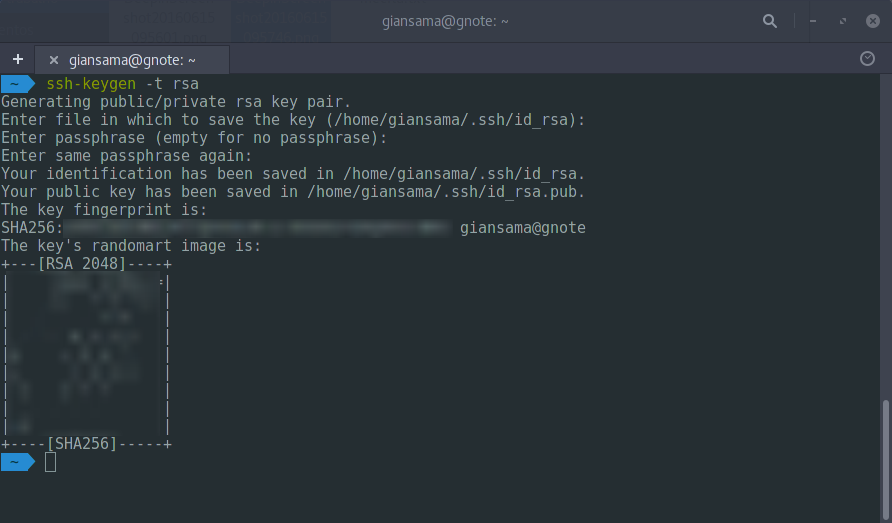
\includegraphics[scale=0.42]{AAUgraphics/ssh3}
\end{frame}
\begin{frame}{Começando a usar}{Registrando a máquina}
  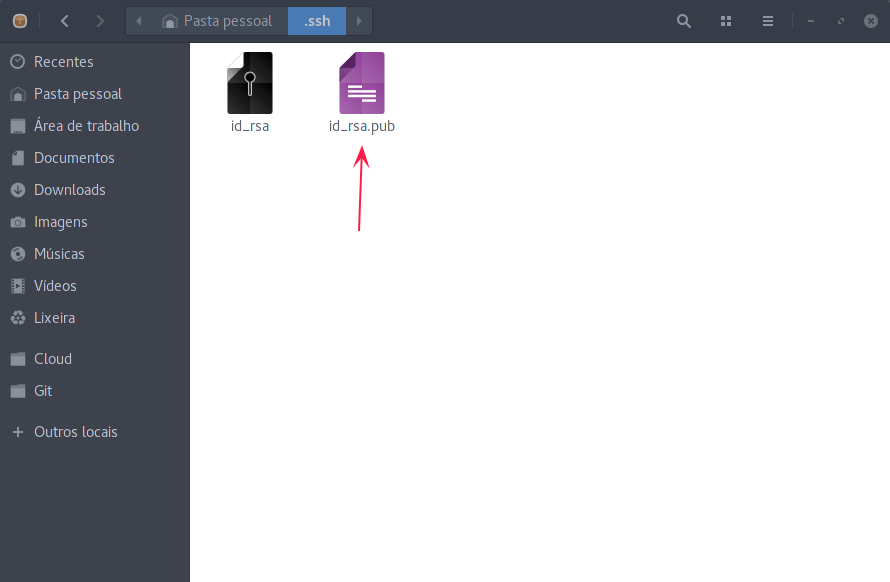
\includegraphics[scale=0.42]{AAUgraphics/ssh4}
\end{frame}
\begin{frame}{Começando a usar}{Registrando a máquina}
  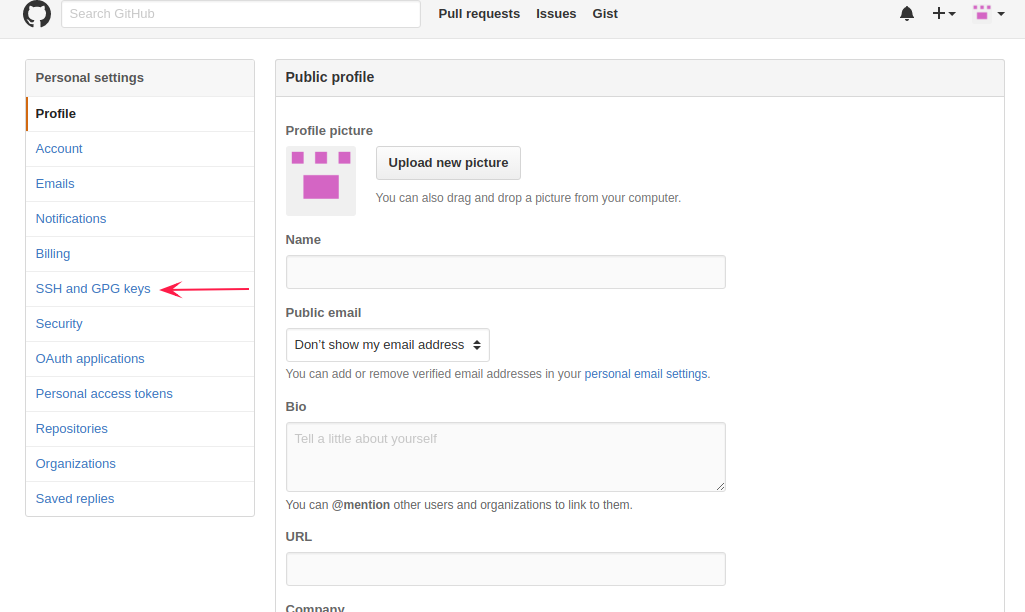
\includegraphics[scale=0.37]{AAUgraphics/ssh5}
\end{frame}
\begin{frame}{Começando a usar}{Registrando a máquina}
  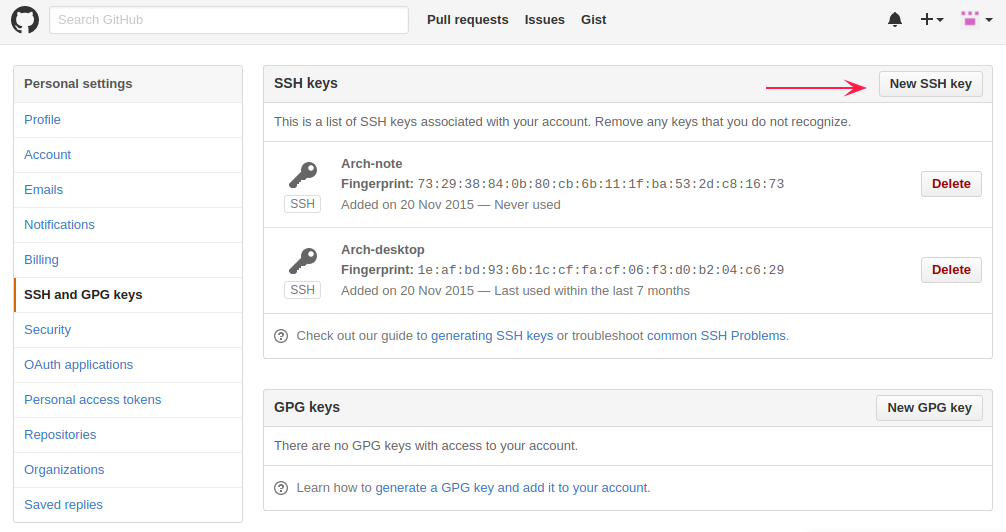
\includegraphics[scale=0.37]{AAUgraphics/ssh6}
\end{frame}

\subsection{Clonando}
\begin{frame}{Começando a usar}{Clonando um repositório}
	Tem 3 formas de clonar um repositório.
	\begin{itemize}
		\item Clonando um repositório local.
		\begin{itemize}
			\item \$ git clone /caminho/para/o/repositório		
		\end{itemize}
		\item Clonando um repositório remoto tendo sabendo nome do usuário, servidor e
				nome do repositório a ser clonado.
		\begin{itemize}
			\item \$ git clone usuário@servidor:/caminho/para/o/repositório		
		\end{itemize}
	\end{itemize}
\end{frame}
\begin{frame}{Começando a usar}{Clonando um repositório}
	\begin{itemize}
	\item Clonando um repositório pelo link do servidor.
	\begin{itemize}
		\item \$ git clone \textit{link do repositório}
	\end{itemize}
	\end{itemize}
	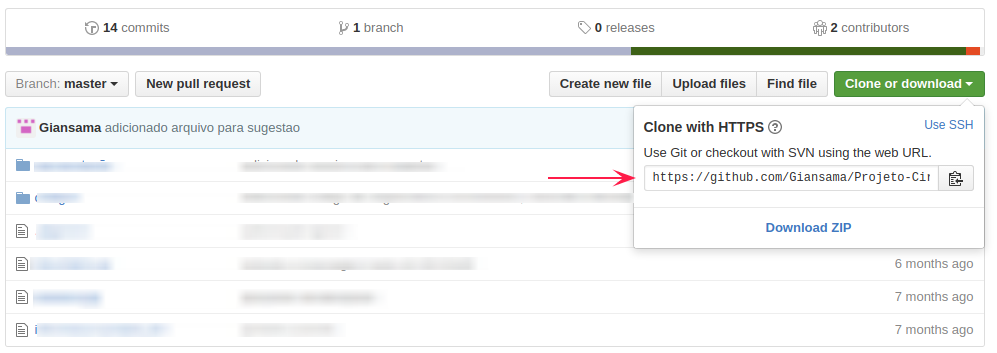
\includegraphics[scale=0.38]{AAUgraphics/clone1}\\
	
\end{frame}

\subsection{Branchs e Forks}
\begin{frame}{Começando a usar}{Manipulando repositórios}
\begin{block}{O que é uma Branch? E o que é um Fork?}
  \begin{itemize}
    \item<1-> Uma Branch é como o nome sugere um 'galho', criar um 'galho' do seu projeto significa ramificar o seu projeto e fazer trabalhos paralelos em cima do mesmo projeto sem que o desenvolvimento de um interfira noutro.\\
    Ao criar uma Branch você criar uma versão paralela do seu projeto aonde você pode trabalhar em alguma alteração sem que isso comprometa a integridade dos arquivos principais. 
    \item<1-> Enquanto um Fork é uma bifurcação do projeto, criar um fork significa levar o projeto para uma direção diferente da que ele esta seguindo agora.\\
    Ao criar uma Fork o projeto é clonado integralmente para um novo repositório e sem qualquer ligação com o original.
  \end{itemize}
\end{block}
\end{frame}

\begin{frame}{Começando a usar}{Criando uma Branch e Merge}
A forma mais rápida de se criar uma branch é pelo comando:
\begin{itemize}
	\item \$ git checkout -b \textit{nome\_da\_branch}
\end{itemize}
Esse comando é na verdade uma simplificação de:
\begin{itemize}
	\item \$ git branch \textit{nome\_da\_branch}
	\item \$ git checkout \textit{nome\_da\_branch}
\end{itemize}
\vspace{10px}
\begin{itemize}
	\item O comando checkout serve para alternar entre as branchs.\\
	\item Para deletar uma branch criada você pode usar:
	\begin{itemize}
		\item {\small \$ git branch -D \textit{nome\_da\_branch}}
	\end{itemize}
	\item Para juntar um ramo a outro é usado o comando merge, estando no ramo que você quer que recebe um outro é só usar o comando:\\
	\begin{itemize}
		\item {\small \$ git merge \textit{nome\_da\_branch}}
	\end{itemize}
\end{itemize}
\end{frame}

\begin{frame}{Começando a usar}{Criando um Fork}
Na verdade o fork não é nada mais que um clone, só que ele é automaticamente rastreado pelo github.
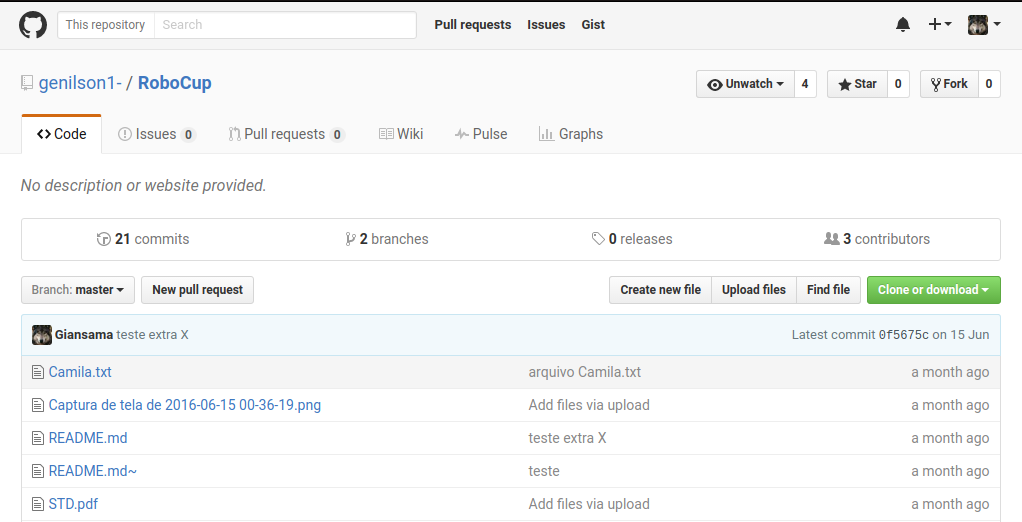
\includegraphics[scale=0.27]{AAUgraphics/fork}
\end{frame}


\section{Comandos}
% general installation instructions
\subsection{Principais comandos}
\begin{frame}{Comandos}{Principais comandos}
Comandos mais comumentes usados:
	\begin{itemize}	
	\item add			
	\item commit			
	\item push			
	\item pull
	\end{itemize}	
\begin{flushright}
{\footnotesize Todos os comandos devem ser iniciados com git + \textit{"comando"}}
\end{flushright}
\end{frame}

%\subsection{Principais comandos}
%\begin{frame}{Comandos}{Outros comandos}%
%	\begin{tabular}{|c|c|}
%		\hline
%		\multicolumn{2}{|c|}{git \textit{comando}}\\
%		\hline
%		clone & \\
%		\hline		
%		add & \\
%		\hline	
%		commit & \\
%		\hline	
%	\end{tabular}
%\end{frame}

%\section{Considerações finais}
%\subsection{Informações dos componentes}
% contact information
%\begin{frame}{Finalizações}{Informações dos componentes}

%\begin{tabular}{lr}
%  Gian Lucas Cavalcante de Lima & 2012919250\\
%\end{tabular}
%
%\end{frame}
%%%%%%%%%%%%%%%%

{\aauwavesbg%
\begin{frame}[plain,noframenumbering]%
  \finalpage{FIM!}
\end{frame}}

\section*{Bonus}
\begin{frame}{BONUS}{Editor de Markdown}
O README no github é um arquivo usado como página em cada repositório e esse arquivo é escrito em markdown(extensão .md).\\
O markdown tem varios códigos chaves que são usados para formatação do texto apresentado. Uma ferramenta que pode ser usada para ajudar a escrever um README mais elaborado e organizado é o Haroopad que pode ser baixado em\\ \begin{center}
\url{http://pad.haroopress.com}
\end{center}
\end{frame}
%%%%%%%%%%%%%%%%

\end{document}
